\section{Auswertung}
\label{sec:Auswertung}
\begin{figure}
	\centering
	\caption{Die Temperatur, am fernem Thermoelement des breiten Messingstabes, $T1$ und, am fernem Thermoelement des schmalen Messingstabe,s $T4$ gegen die vergangene Zeit $t$ aufgetragen.}
	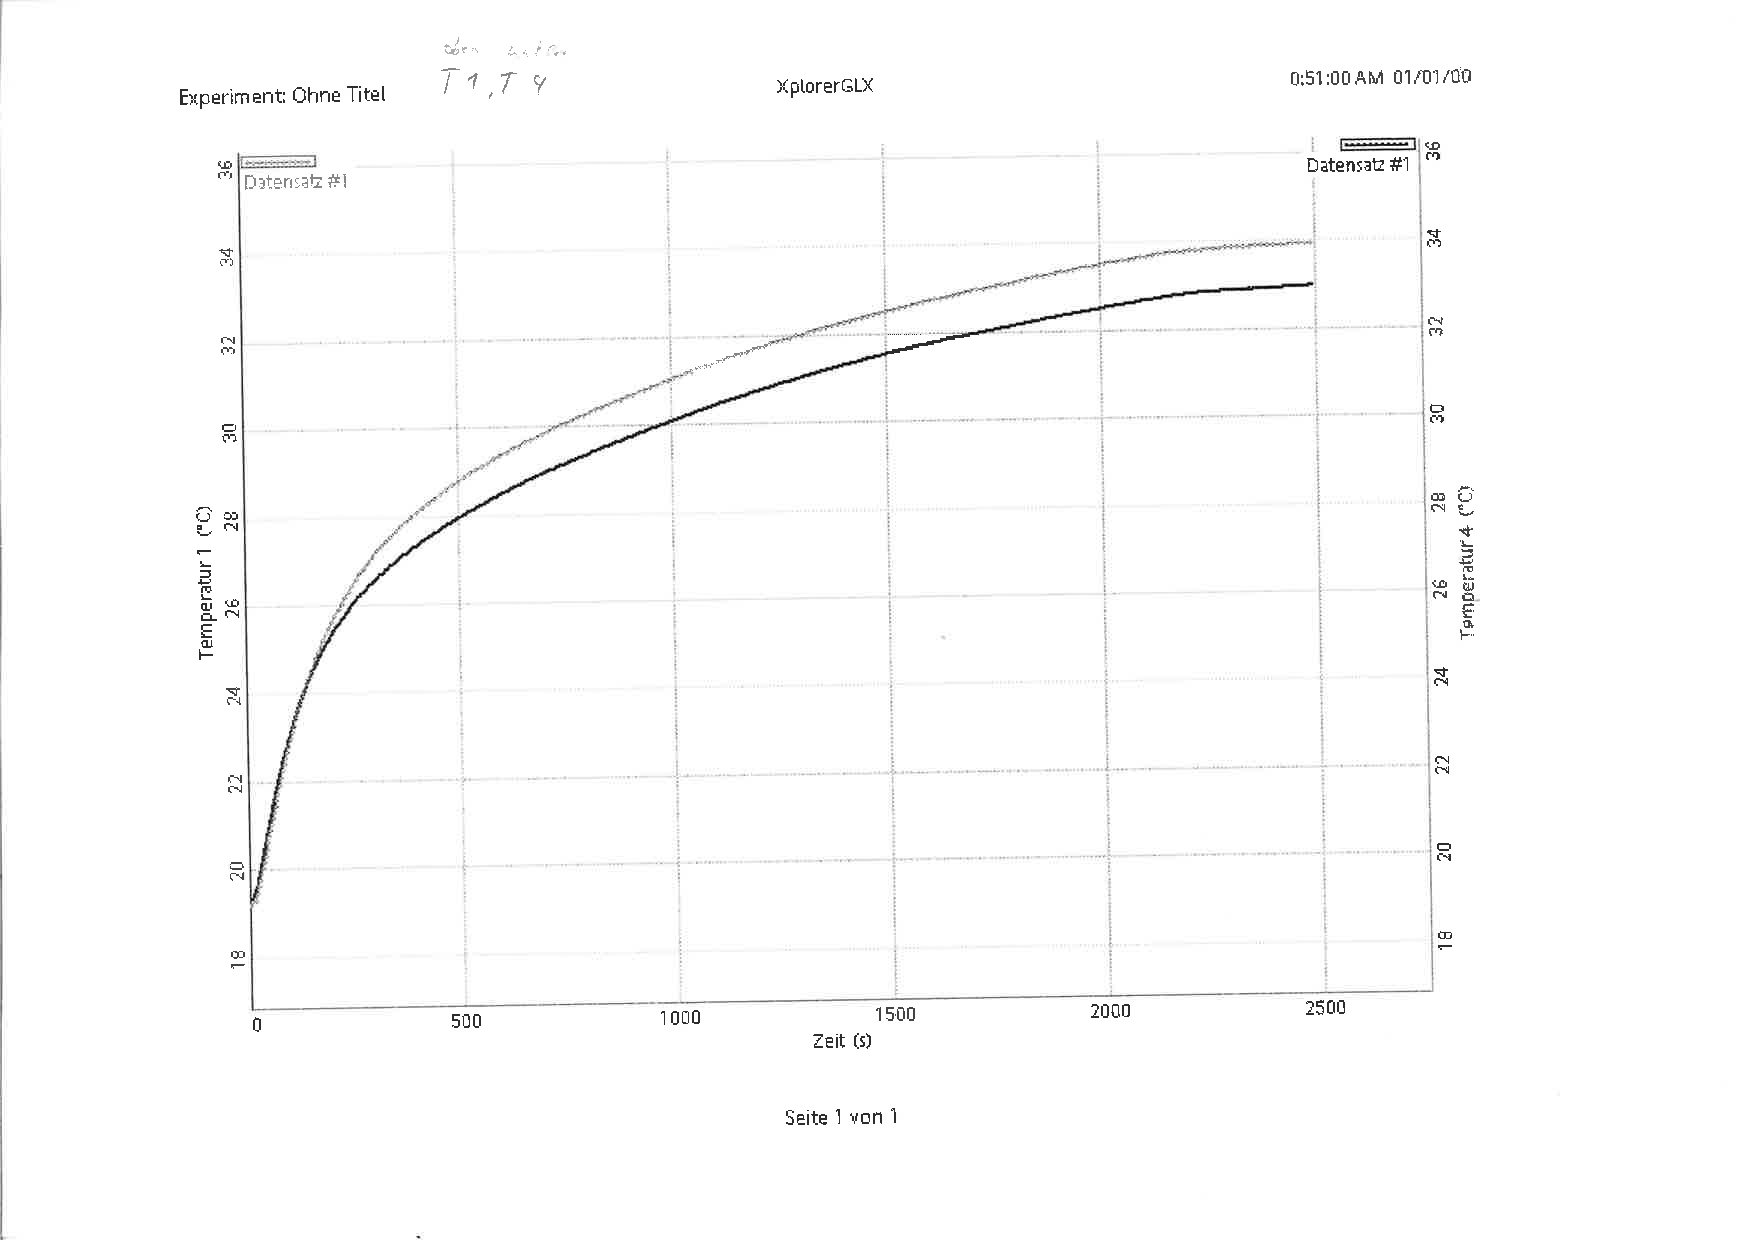
\includegraphics[width=\linewidth-70pt,height=\textheight-70pt,keepaspectratio]{content/Bilder/T1T4-rotated.pdf}
	\label{fig:Graph1}
\end{figure}
\begin{figure}
	\centering
	\caption{Die Temperatur, am fernem Thermoelement des Aluminiumstabes, $T5$ und, am fernem Thermoelement des Edelstahlstabes, $T8$ gegen die vergangene Zeit $t$ aufgetragen.}
	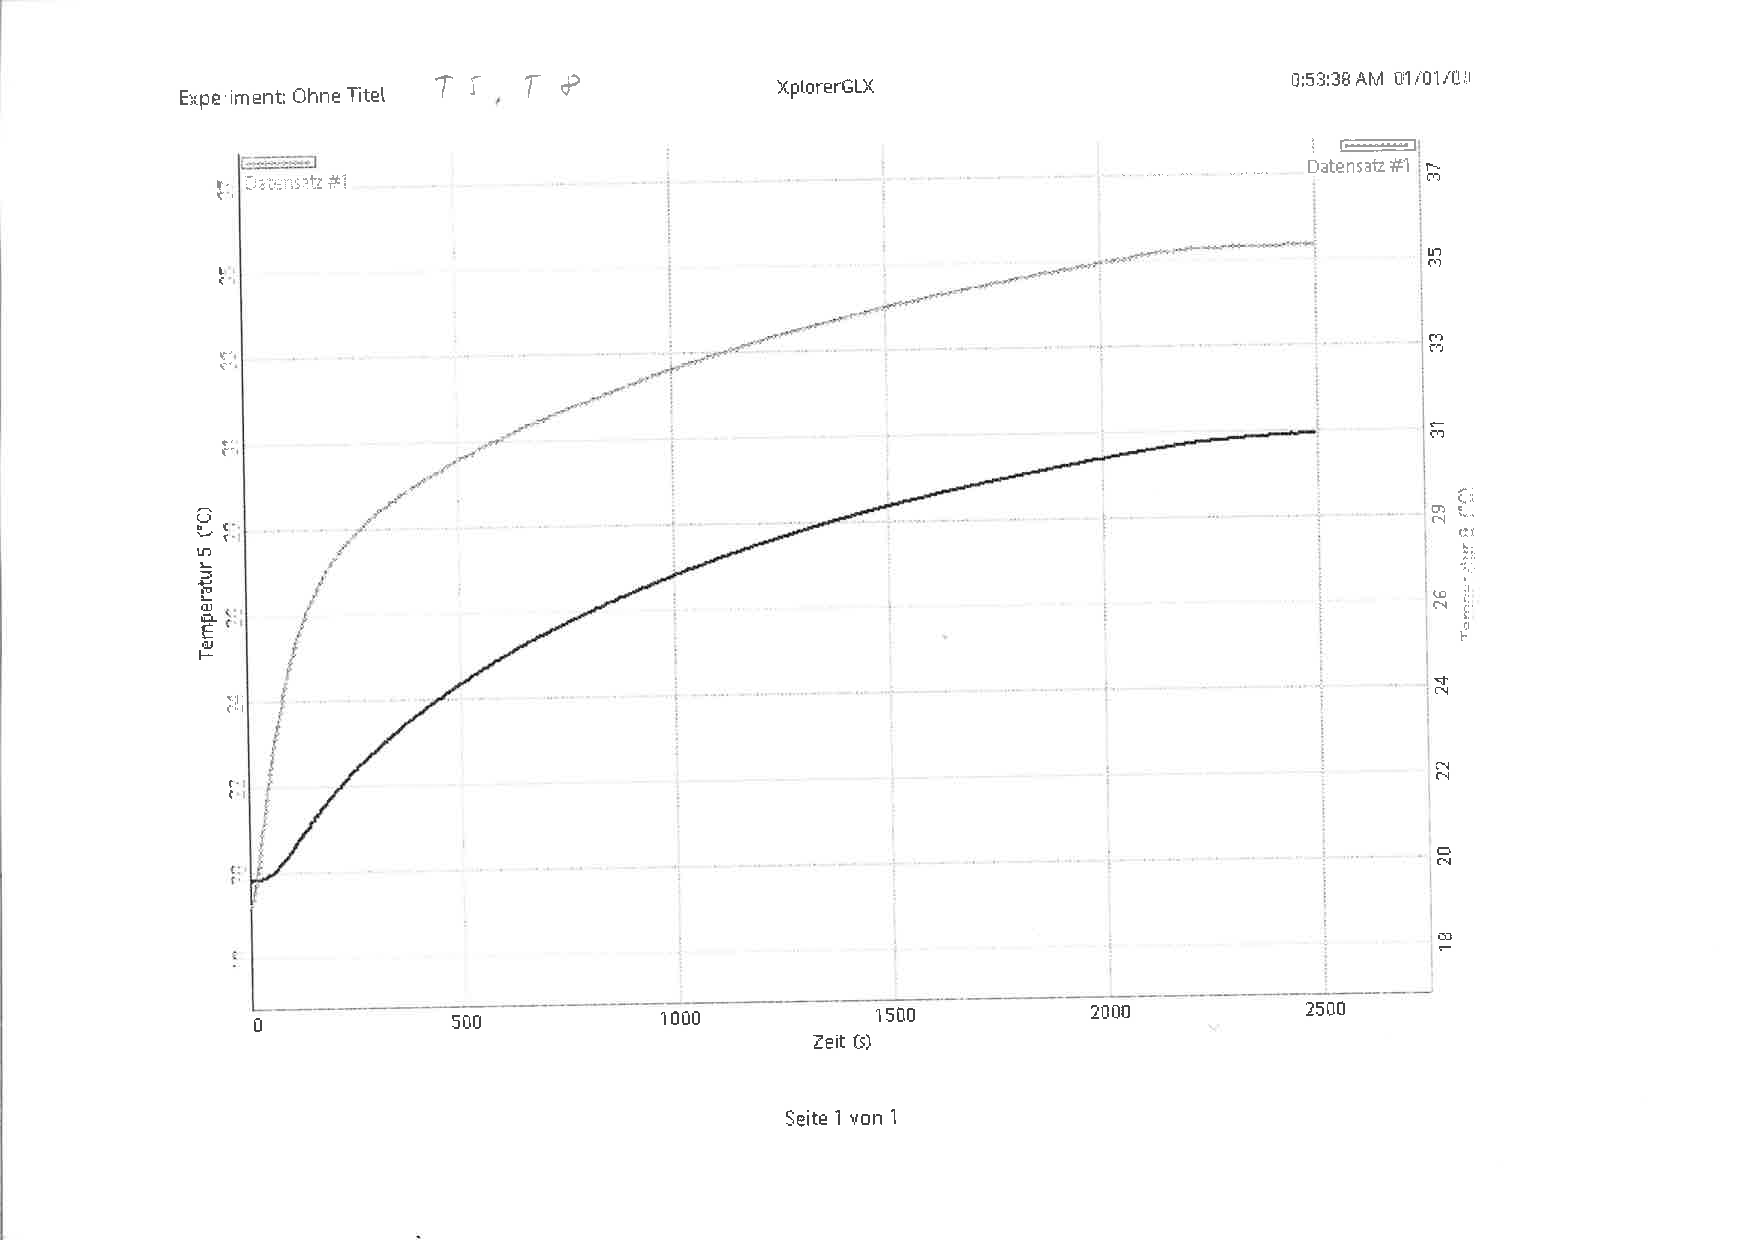
\includegraphics[width=\linewidth-70pt,height=\textheight-70pt,keepaspectratio]{content/Bilder/T5T8-rotated.pdf}
	\label{fig:Graph2}
\end{figure}
\begin{figure}
	\centering
	\caption{Die Temperaturdifferenz $T2-T1$ bei dem breitem Messingstab gegen die vergangene Zeit $t$ aufgetragen.}
	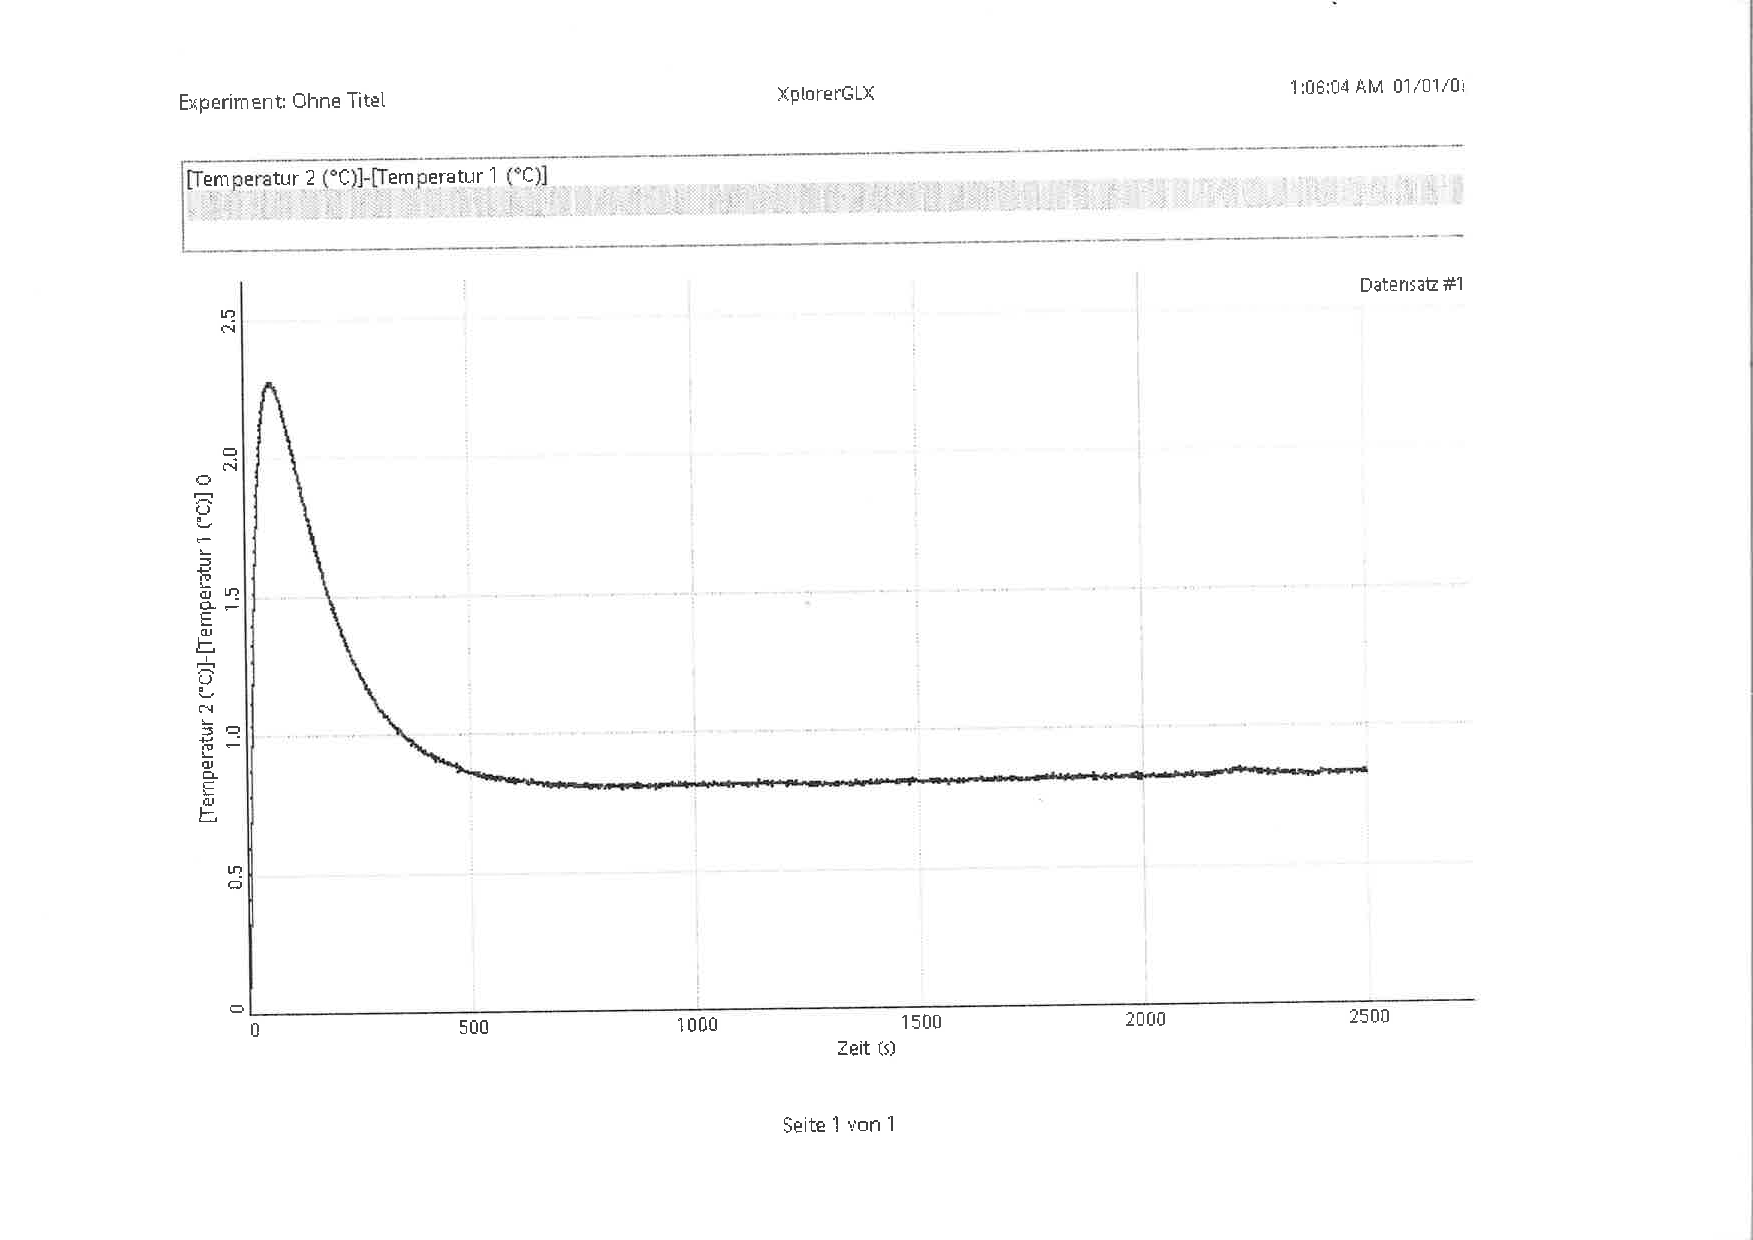
\includegraphics[width=\linewidth-70pt,height=\textheight-70pt,keepaspectratio]{content/Bilder/T2-T1-rotated.pdf}
	\label{fig:Graph3}
\end{figure}
\begin{table}
	\centering
	\caption{Der nach Formel \eqref{eq:form1} berechnete Wärmestrom $\frac{\Delta Q_{21}}{\Delta t}$ nach der Zeit $t$ und die aus \ref{fig:Graph3} entnommene Temperaturdifferenz $T2-T1$ bei dem breitem Messingstab.}
	\input{./build/tabT21.tex}
\end{table}
\begin{figure}
	\centering
	\caption{Die Temperaturdifferenz $T7-T8$ bei dem Edelstahlstab gegen die vergangene Zeit $t$ aufgetragen.}
	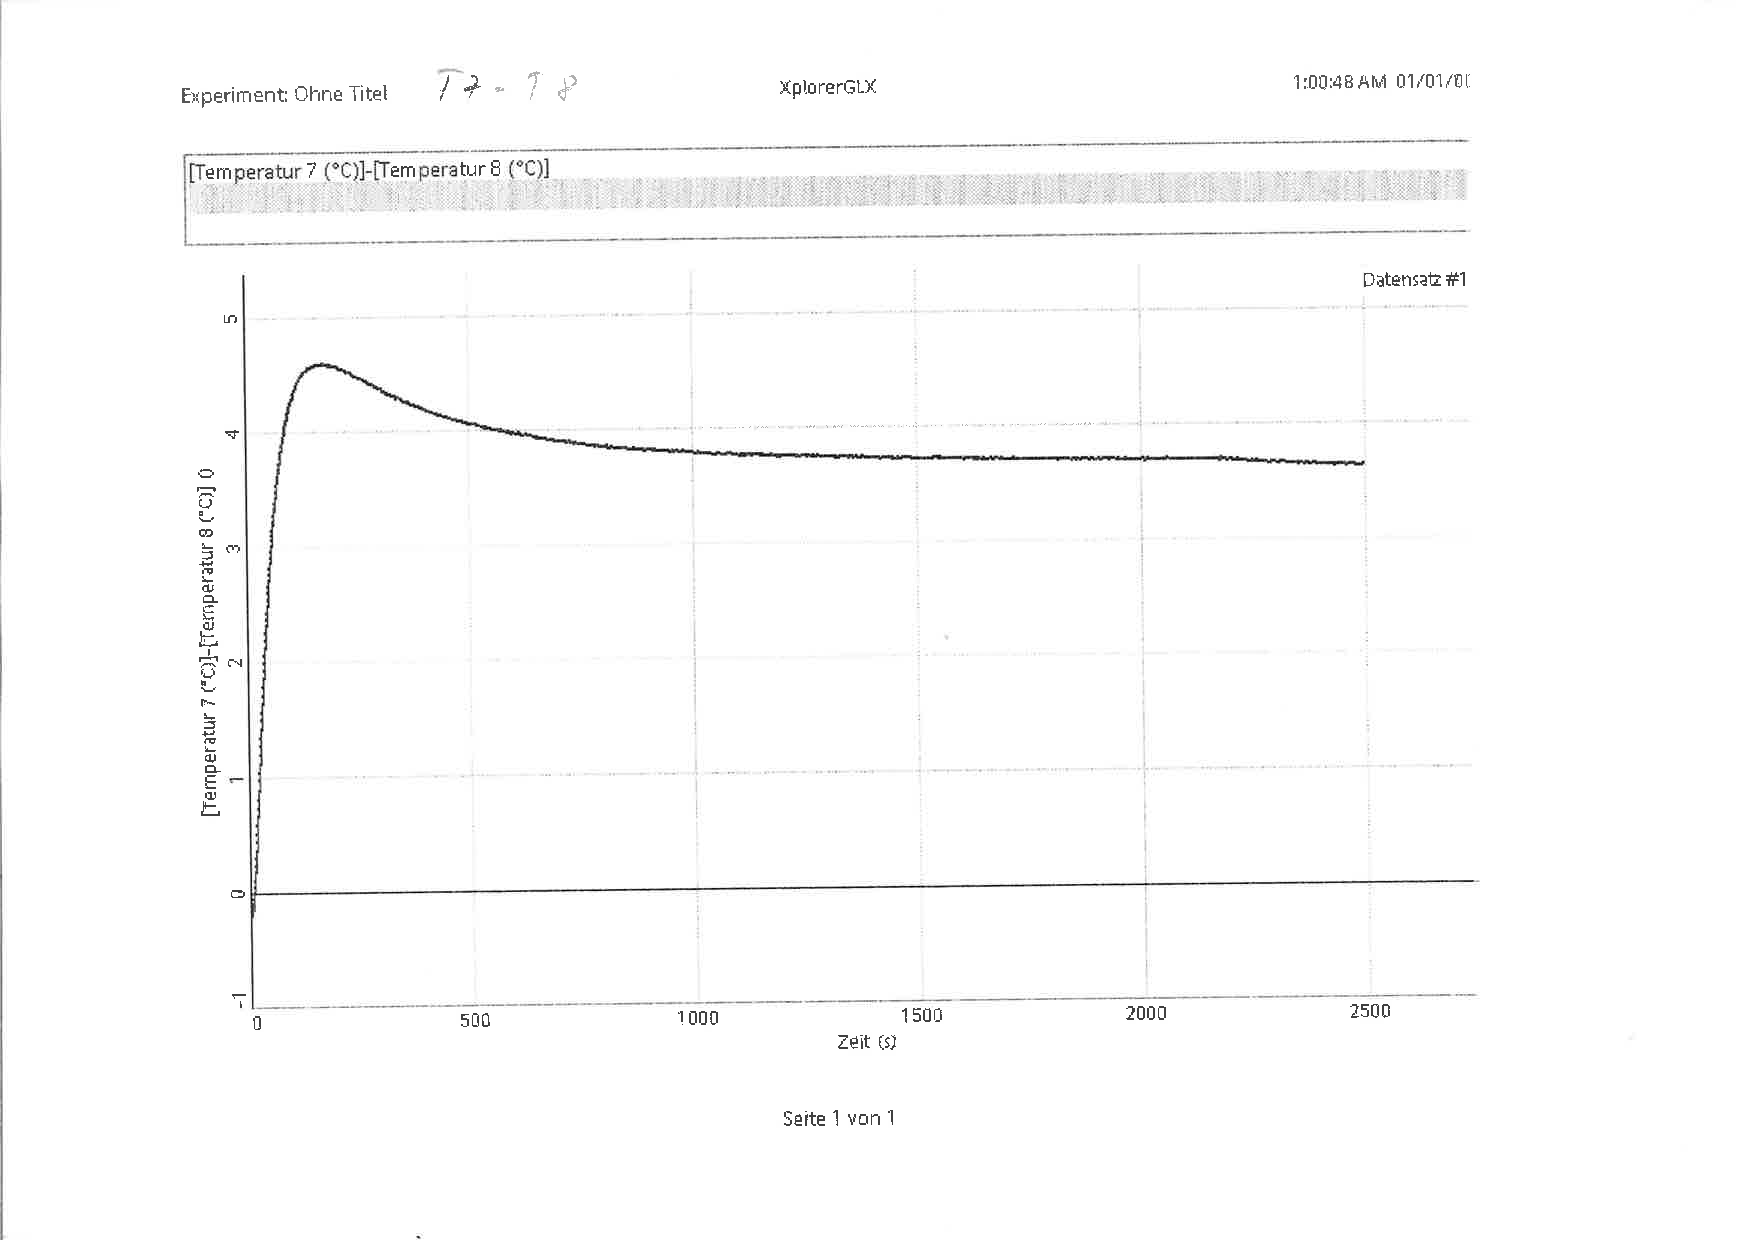
\includegraphics[width=\linewidth-70pt,height=\textheight-70pt,keepaspectratio]{content/Bilder/T7-T8-rotated.pdf}
	\label{fig:Graph4}
\end{figure}
\begin{table}
	\centering
	\caption{Der nach Formel \eqref{eq:form1} berechnete Wärmestrom $\frac{\Delta Q_{78}}{\Delta t}$ nach der Zeit $t$ und die aus \ref{fig:Graph4} entnommene Temperaturdifferenz $T7-T8$ bei dem Edelstahlstab.}
	\input{./build/tabT78.tex}
\end{table}
\begin{figure}
	\centering
	\caption{Die Temperatur, am nahem Thermoelement des Messingstabes, $T2$ und, am fernem Thermoelement, $T1$ gegen die vergangene Zeit $t$ aufgetragen.}
	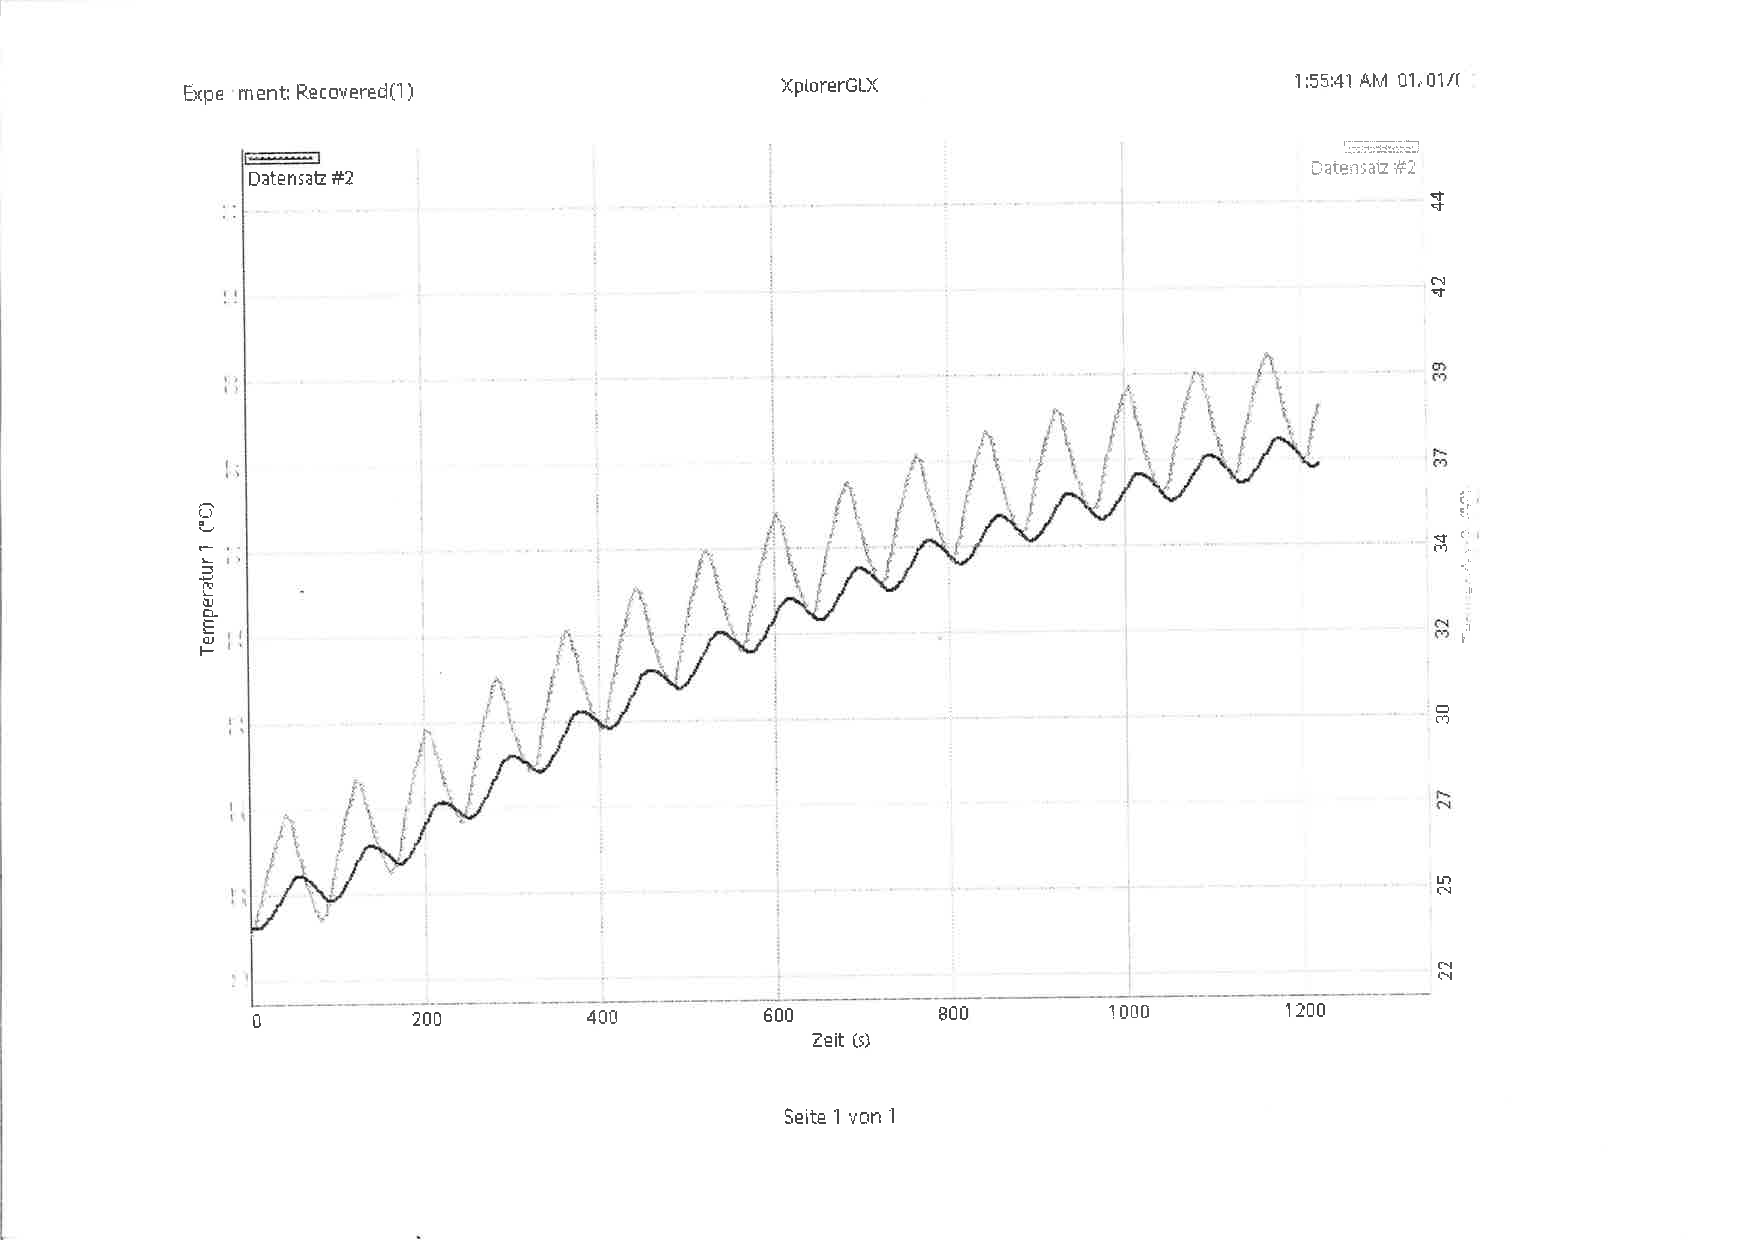
\includegraphics[width=\linewidth-70pt,height=\textheight-70pt,keepaspectratio]{content/Bilder/T1T2-rotated.pdf}
	\label{fig:Graph5}
\end{figure}
\begin{table}
	\centering
	\caption{Die aus dem Graphen in Abbildung \ref{fig:Graph5} entnommenen Werte für die Phasendifferenz $\Delta t$ die Amplitude am nahem Thermoelement des breitem Messingstabes $A_\text{nah}$ und am fernem Thermoelement $A_\text{fern}$.}
	\input{./build/tabMessing.tex}
\end{table}
\begin{figure}
	\centering
	\caption{Die Temperatur, am nahem Thermoelement des Aluminiumstabes, $T6$ und, am fernem Thermoelement, $T5$ gegen die vergangene Zeit $t$ aufgetragen.}
	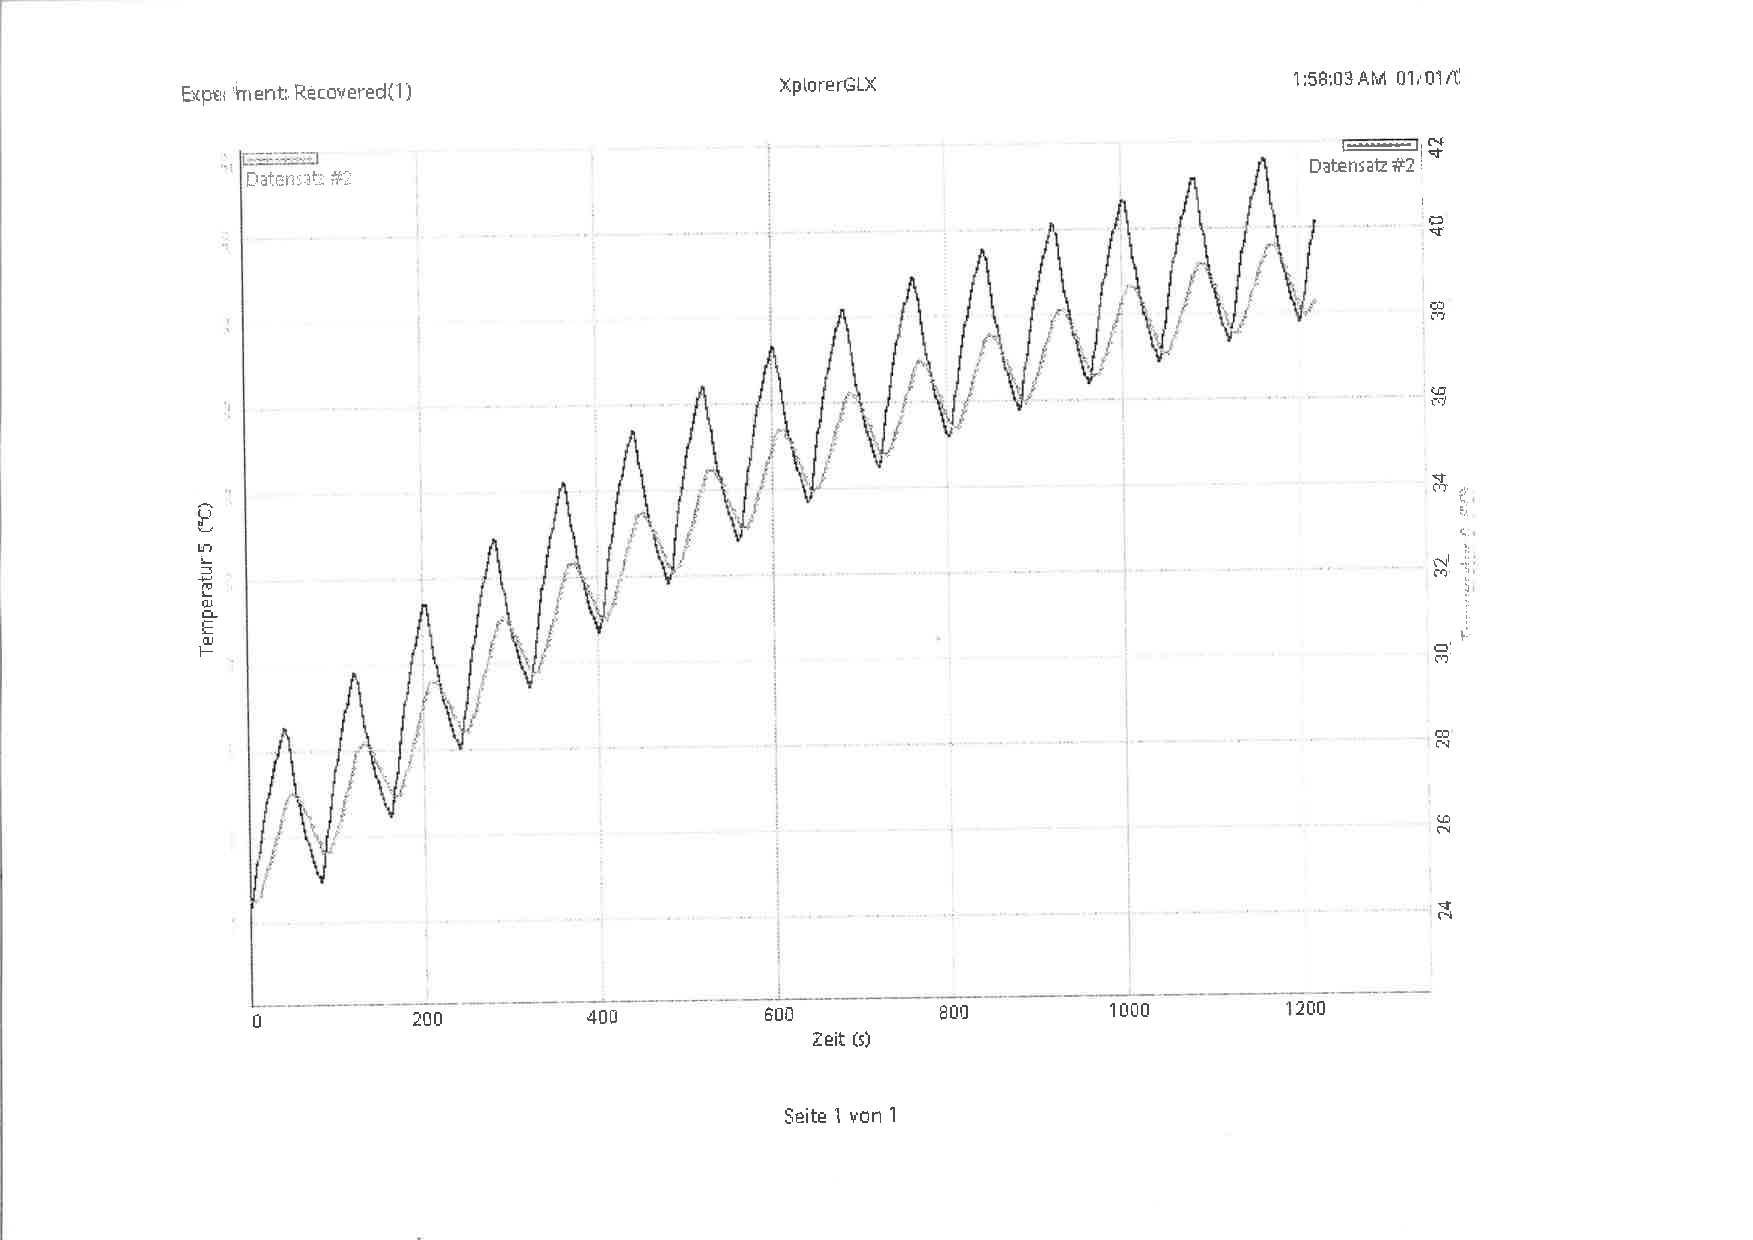
\includegraphics[width=\linewidth-70pt,height=\textheight-70pt,keepaspectratio]{content/Bilder/T5T6-rotated.pdf}
	\label{fig:Graph6}
\end{figure}
\begin{table}
	\centering
	\caption{Die aus dem Graphen in Abbildung \ref{fig:Graph6} entnommenen Werte für die Phasendifferenz $\Delta t$ die Amplitude am nahem Thermoelement des Aluminiumstabes $A_\text{nah}$ und am fernem Thermoelement $A_\text{fern}$.}
	\input{./build/tabAluminium.tex}
\end{table}
\begin{figure}
	\centering
	\caption{Die Temperatur, am nahem Thermoelement des Edelstahlstabes, $T7$ und, am fernem Thermoelement, $T8$ gegen die vergangene Zeit $t$ aufgetragen.}
	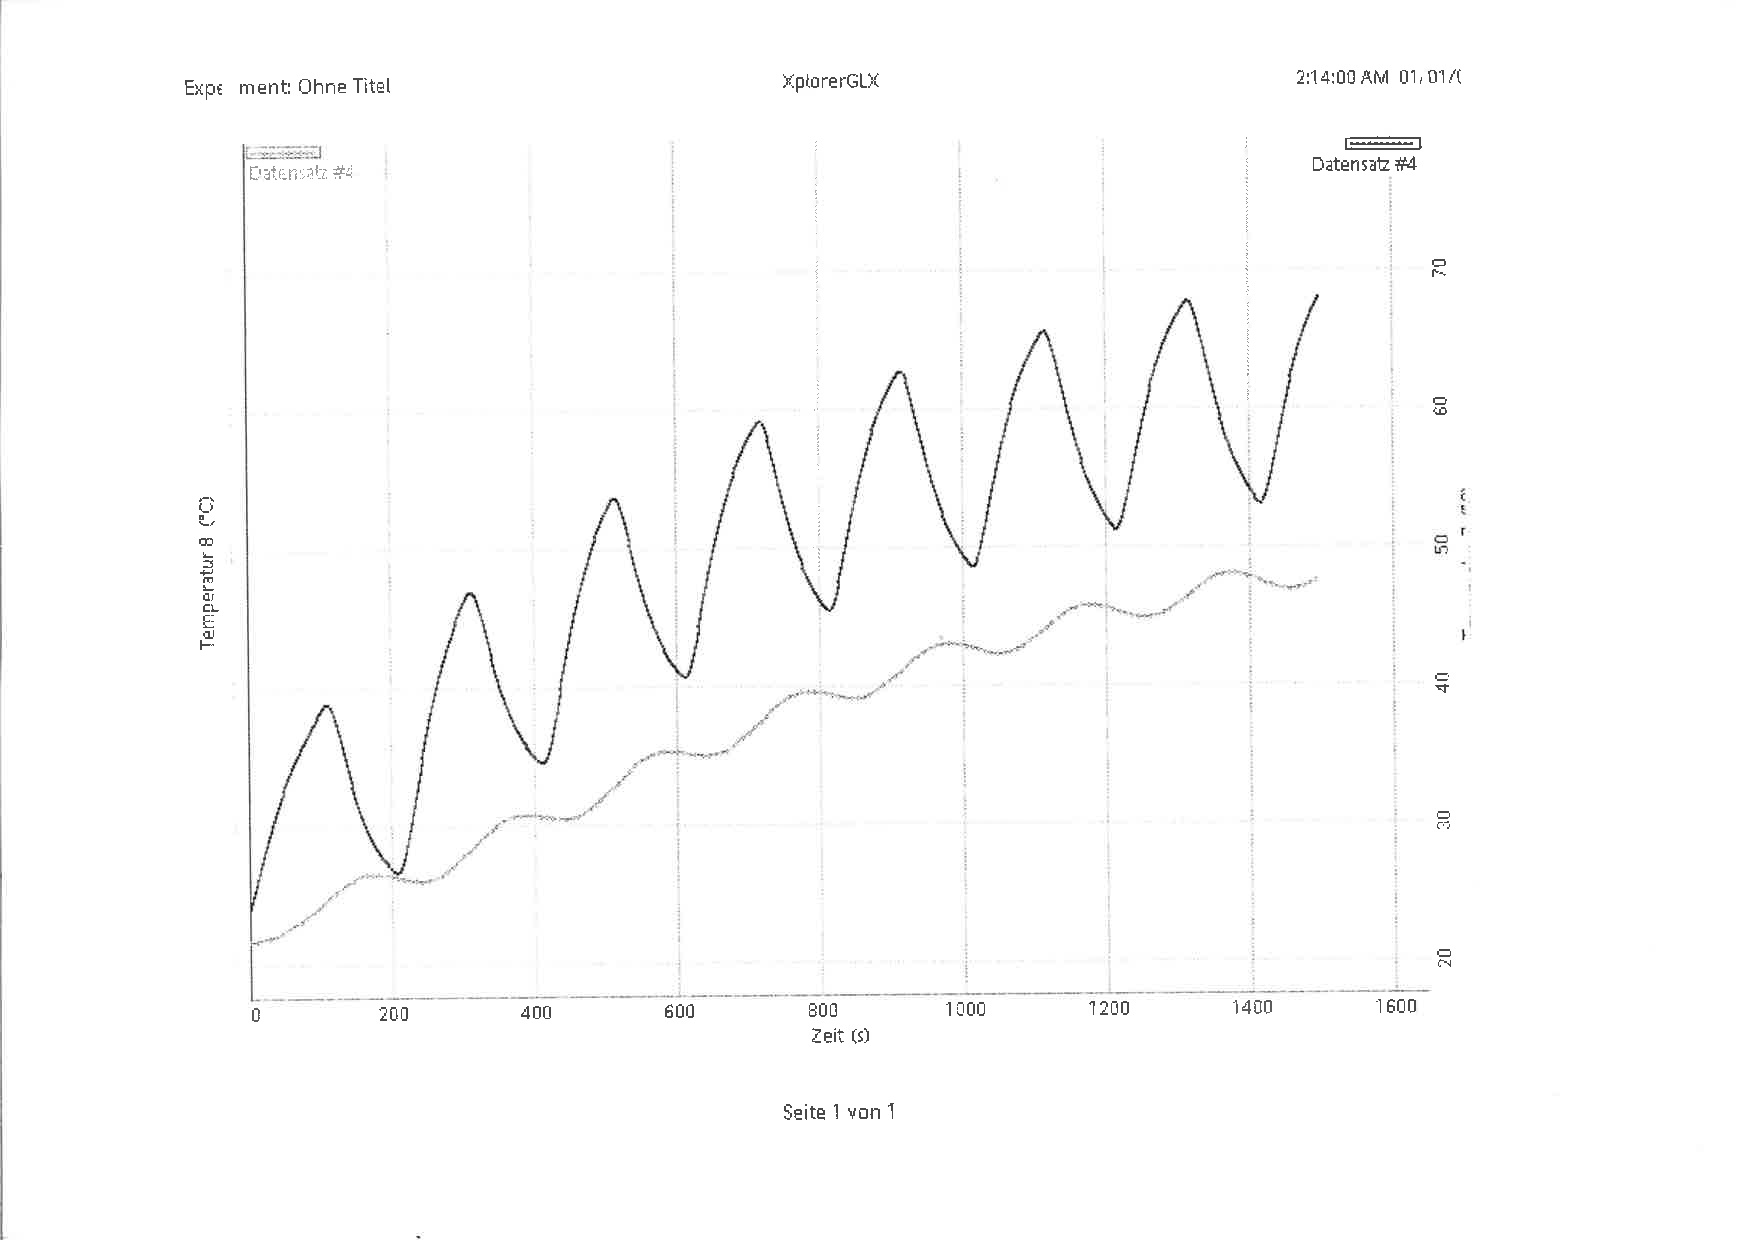
\includegraphics[width=\linewidth-70pt,height=\textheight-70pt,keepaspectratio]{content/Bilder/T7T8-rotated.pdf}
	\label{fig:Graph7}
\end{figure}
\begin{table}
	\centering
	\caption{Die aus dem Graphen in Abbildung \ref{fig:Graph7} entnommenen Werte für die Phasendifferenz $\Delta t$ die Amplitude am nahem Thermoelement des Edelstahlstabes $A_\text{nah}$ und am fernem Thermoelement $A_\text{fern}$.}
	\input{./build/tabEdelstahl.tex}
\end{table}